\documentclass[aps,prd,onecolumn,nofootinbib,letterpaper,preprintnumbers,superscriptaddress,eqsecnum]{revtex4}

\usepackage[utf8]{inputenc}
\usepackage[english]{babel}
\usepackage{amsfonts}
\usepackage{amssymb}
\usepackage{amsmath}
\usepackage{amsthm}
\usepackage[usenames,dvipsnames]{xcolor}
\usepackage{graphicx}
\usepackage{hyperref}
\usepackage{dsfont}
\usepackage{tikz-cd}
\usepackage{cleveref}
\usepackage{txfonts}
\usepackage{tikz, tikz-cd}
\usepackage{subfigure}
\usepackage[version=4]{mhchem}
\usetikzlibrary{backgrounds,circuits,circuits.ee.IEC,shapes,fit,matrix}

\tikzstyle{arrow}=[-,postaction={decorate},decoration={markings,mark=at position .5 with {\arrow{>}}},line width=1.100]
\pgfdeclarelayer{edgelayer}
\pgfdeclarelayer{nodelayer}
\pgfsetlayers{edgelayer,nodelayer,main}

\tikzstyle{none}=[inner sep=0pt]

\definecolor{lblue}{rgb}{0,250,255}

\tikzstyle{site}=[circle, fill=lblue!20, draw=black, scale=1, minimum size=1cm]
\tikzstyle{catalyst}=[circle, fill=lblue!20, draw=red, scale=1, minimum size=1cm]
\tikzstyle{transition}=[rectangle, fill=gray!30, draw=black, scale=1, minimum size=1cm]
\tikzstyle{morphism}=[rectangle, fill=gray!30, draw=black, scale=1, minimum size=1cm]

\tikzstyle{empty}=[circle, fill=none, draw=none]
\tikzstyle{inputdot}=[circle, fill=black, draw=black, scale=.5]
\tikzstyle{dot}=[circle, fill=black, draw=black]
\tikzstyle{bounding}=[circle, dashed, fill=none, draw=black, scale=9.00]
\tikzstyle{simple}=[->, draw=black, line width=1]
\tikzstyle{arrow}=[-, draw=black, postaction={decorate}, decoration={markings,mark=at position .5 with {\arrow{>}}}, line width=1.000]
\tikzstyle{tick}=[-, draw=black, postaction={decorate}, decoration={markings,mark=at position .5 with {\draw (0,-0.1) -- (0,0.1);}}, line width=1.000]
\tikzstyle{inputarrow}=[->, draw=black, shorten >=.05cm]
\tikzstyle{sitemap}=[->, dashed, draw=red, ultra thick, shorten >=.05cm]
\tikzstyle{transitionmap}=[->, dashed, draw=blue, ultra thick, shorten >=.05cm]


\newtheorem{lemma}{Lemma}
\newtheorem{corollary}{Corollary}
\newtheorem{theorem}{Theorem}

\theoremstyle{definition}
\newtheorem{definition}{Definition}

\newcommand{\upset}[1]{#1\!\!\uparrow}
\newcommand{\downset}[1]{#1\!\!\downarrow}
\newcommand{\N}{\mathbb{N}}
\newcommand{\B}{\mathcal{B}}
\newcommand{\G}{\mathcal{G}}
\newcommand{\Ini}[1]{\textrm{Ini}(#1)}
\newcommand{\Term}[1]{\textrm{Term}(#1)}
\newcommand{\A}{\mathcal{A}}
\newcommand{\powerset}{\mathcal{P}}
\newcommand{\pathway}[1]{\langle#1\rangle}
\newcommand{\R}{\mathbb{R}}

\newcommand{\red}[1]{{\color{red}#1}}
\newcommand{\green}[1]{{\color{ForestGreen}#1}}
\newcommand{\blue}[1]{{\color{blue}#1}}
\newcommand{\TODO}[1]{\noindent\red{\textbf{TODO:}~#1}}

\begin{document}

\title{Supplementary Information: Quantifying the pathways to life using assembly spaces}
\author{Stuart M. Marshall}
\author{Douglas G. Moore}
\author{Alastair R. G. Murray}
\author{Sara I. Walker}
\author{Leroy Cronin}

\maketitle

\section{Introduction}

This formalism arose as a means of rigorously describing the ``simplest" way of assembling a given object by combining basic building blocks.
With this in mind, we consider a universe of objects together with transitions representing ways in which objects can be combined, mutated or disassembled to yield other objects.
In this setting, the concrete rules or laws relating the transitions with the objects is largely neglected herein, though they are certainly necessary for initially constructing the space for consideration.
We quickly come to the conclusion that a Petri network is appropriate when we consider this kind of process in general, though with specific modifications to allow the types of questions in which we are interested to be well defined.
As such, the fundamental mathematical structure we define and explore herein, referred to as an assembly space, can be described as a sourceless, sinkless Petri net with a chosen basis.
The details of this description will, of course, be made precise below.
With assembly spaces defined, we are then able to define an assembly index for each object in the space, relative to the chosen basis, which characterizes how directly that object can be assembled.
Further, we prove several theorems relating to method of bounding the assembly index for a given object and algorithms for computing or approximating it.

[This is Sara testing if she can git cool like the rest of the peeps in elife, I will remove on my next commit]

\section{Petri Nets}

\subsection{Free Commutative Monoids}\label{subsec:fcm}

The first task we are faced with is how to formally represent the substrates and products of some transition.
We can look to introductory Chemistry for inspiration.
When we consider a process like
\begin{equation*}
    \ce{2H_2} + \ce{O_2} \rightarrow \ce{2H_2O}
\end{equation*}
we are expressing the idea that some chemical process (transition) consumes twice as much $\ce{H_2}$ as $\ce{O_2}$ and yields $\ce{H_2O}$.
The apparent multiplication ($\ce{2H_2}$) and addition ($\ce{2H_2} + \ce{O_2}$) are simply formal constructs use to encode the stoichiometry of the reaction.
The addition here is commutative; we could have written $\ce{O_2} + \ce{2H_2}$, and it would have meant precisely the same thing.

We take a similar approach herein, though mathematically explicit. Let $X$ be a set. This may be, for example, a set of types of molecules $\{\ce{H_2}, \ce{O_2}, \ce{H_2O}\}$ or a set of kinds of building materials and products $\{\textrm{wood}, \textrm{glass pane}, \textrm{nail}, \textrm{picture frame}\}$.
We can then construct formal linear combinations of the elements of $X$ where the coefficients are natural numbers, e.g. $\ce{2H_2} + \ce{O_2}$ or $4\textrm{wood} + \textrm{glass pane} + 8\textrm{nail}$, and only finitely many coefficients are nonzero.

The collection of such formal linear combinations is referred to as the \textit{free commutative monoid} on $X$ over the natural number $\N$, and is typically denoted $\N[X]$.
The set $X$, in this context, is referred to as the set of generators of $\N[X]$.
An element $a \in \N[X]$ can be written as
\begin{equation*}
    a = \sum_{x \in X} a_x x
\end{equation*}
with natural number coefficients $a_x$, only finitely many non-zero.
This construction naturally has a monoidal structure, hence the name.
You can add such linear combinations together, e.g. $\ce{H_2} + (\ce{H_2} + \ce{O_2}) = \ce{2H_2} + \ce{O_2}$, and there exists an identity element $0$ such that $0 + a = a + 0 = a$ for all $a \in \N[X]$.
It is important to stress at this point that the linear combinations do not need to ``make sense'', at least not yet.
Taking the molecular example, $\ce{H_2}$, $\ce{7H_2} + \ce{O_2}$ and $\ce{H_2} + \ce{H_2O} + \ce{O_2}$ are permissible linear combinations and so they are elements of $\N[X]$.
This does not mean that we will, in practice, consider all of them.
Restrictions on which linear combinations are consider will come into the picture when we introduce transitions.

For some of the definitions we will present in coming sections, it will be useful to denote the subset of generators appearing in a given linear combinations. That is for a given element $a \in \N[X]$, the subset generators with non-zero coefficients in $a$, denoted $\pi : \N[X] \rightarrow \powerset{X}$ where
\begin{equation*}
    \displaystyle \sum_{x \in X} a_x x \mapsto \{ x \in X ~|~ a_x \ne 0 \}.
\end{equation*}
To clarify this point, $\pi(\ce{2H2} + \ce{O_2}) = \{\ce{H_2}, \ce{O_2}\}$.

\red{Describe the relationship between the $\pi$ notation and the addition operator since we use both in subsequent sections.}

Before departing from the topic of the free commutative monoid, we want to note that while it may seem that we are being overly formalistic, we gain some power by taking this approach.
Most importantly, we can consider what happens if you ``map'' one set of objects into another.
As a concrete example, you could imagine mapping each of the molecules $\ce{H_2}$, $\ce{O_2}$ and $\ce{H_2O}$ to the number of Hydrogen atoms they contain, i.e. $2$, $0$, and $2$.
\red{I don't like that example very much, but it's good enough for the moment.}
This mapping process can be ``lifted'' into a map on the linear combinations by distributing the map over addition, so that $\ce{H_2} + \ce{O_2}$ maps to $2 + 0 = 2$. More formally, any function between sets $f : X \rightarrow Y$ can be uniquely extended to a function $\N[f] : \N[X] \rightarrow \N[Y]$ such that
\begin{equation*}
    \sum_{x \in X} a_x x \mapsto \sum_{x \in X} a_x f(x).
\end{equation*}
The value of doing this is that it will allow us to coherently define a map between assembly spaces, to be defined, which will then be useful for proving certain theorems regarding bounds on quantities of interest.

\subsection{Petri Nets}

We wish to represent the idea of assembling objects out of ``simpler'' objects, in some sense of the word.
To formalize this idea, we will build off of the concept of a \textit{Petri net}.
In simple terms, a Petri net is a set of sites which we think of as representing types of objects, e.g. molecules, building materials, characters, etc..., and a set of transitions representing the ways in which sites can be combined to yield other sites.
For the sake of formalism, we somewhat elevate the transitions above the sites in that we mostly consider the ``inputs'' and ``outputs'' of transitions, rather the transitions that a given site participates in.
With this in mind, we formally define a Petri net as follows.

\begin{definition}\label{def:petri}
    A \textbf{Petri net} is a $P$ consisting of
    \begin{itemize}
        \item a set of \textit{sites}, $S(P)$
        \item a set of \textit{transitions}, $T(P)$
        \item a pair of maps $\begin{tikzcd}
                T(P)
                \arrow[r, shift left = 1, "\sigma_P"]
                \arrow[r, shift right = 1, "\tau_P", swap]
                &
                \N[S(P)]
        \end{tikzcd}$.
    \end{itemize}
    We call $\sigma_P$ the source map and $\tau_Q$ the target map.
    Where context is unambiguous we may simply write $\sigma$ and $\tau$, but will generally retain the $T(P)$ and $S(P)$ notation.
\end{definition}

The maps $\sigma$ and $\tau$ assign to each transition a formal linear combination of sites.
Picking up our molecular example from the previous section, we can consider the Petri net with sites $S = \{\ce{H_2}, \ce{O_2}, \ce{H_2O}\}$, a single transition $T = \{\alpha\}$, and source and target maps
\begin{equation*}
    \begin{tikzcd}
        \alpha \arrow[r, mapsto, "\sigma"] & 2\ce{H_2} + \ce{O_2}
        \quad\textrm{and}\quad
        \alpha \arrow[r, mapsto, "\tau"] & 2\ce{H_2O}
    \end{tikzcd}
\end{equation*}

There is a natural way of graphically representing a Petri net as a bipartite multigraph:

\begin{center}
    \scalebox{0.6}{
        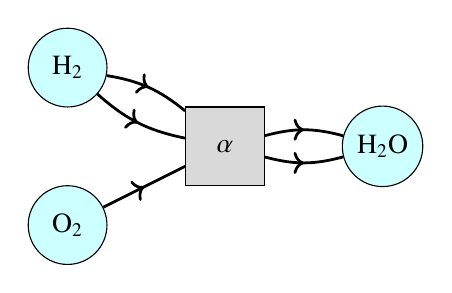
\begin{tikzpicture}
            \begin{pgfonlayer}{nodelayer}
                \node [style=site] (H2) at (0, 1) {$\ce{H_2}$};
                \node [style=site] (O2) at (0, -1) {$\ce{O_2}$};
                \node [style=site] (H2O) at (4, 0) {$\ce{H_2O}$};
                \node [style=transition] (alpha) at (2, 0) {$\alpha$};
            \end{pgfonlayer}
            \begin{pgfonlayer}{edgelayer}
                \draw [style=arrow, bend right=15] (H2) to (alpha);
                \draw [style=arrow, bend left=15] (H2) to (alpha);
                \draw [style=arrow] (O2) to (alpha);
                \draw [style=arrow, bend right=15] (alpha) to (H2O);
                \draw [style=arrow, bend left=15] (alpha) to (H2O);
            \end{pgfonlayer}
        \end{tikzpicture}
    }
\end{center}

We read this as ``\textit{transition $\alpha$ can only proceed if at least two $\ce{H_2}$ and one $\ce{O_2}$ are present in the system, and will yield two $\ce{H_2O}$ when it does}''.
In essence, this is a statement about was can possibly happen, not necessarily what will happen; that's more a question of dynamics.

As a more elaborate example, one which we will repeatedly refer to as we expand on the formalism as it exhibits number of interesting features, we imagine a simple ligation type process where in the characters $A$ and $B$ can be combined into strings and $C$ acts something like a \red{``catalyst''} making some transitions possible if and only if $C$ exists.
Consider the Petri $P$ net described by $S(P) = \{ A, B, C, AA, AB, AAAB \}$ and $T(P) = \{ \alpha, \beta, \gamma, \delta \}$ with source and target maps:

\begin{align*}
    \sigma(\alpha) &= 2A           & \tau(\alpha) &= AA         \\
    \sigma(\beta)  &= A + B        & \tau(\beta)  &= AB         \\
    \sigma(\gamma) &= AA + AB + C  & \tau(\gamma) &= AAAB + C   \\
    \sigma(\delta) &= AAAB         & \tau(\delta) &= A + AA + B
\end{align*}

which we graphically represent as

\begin{center}
    \scalebox{0.6}{
        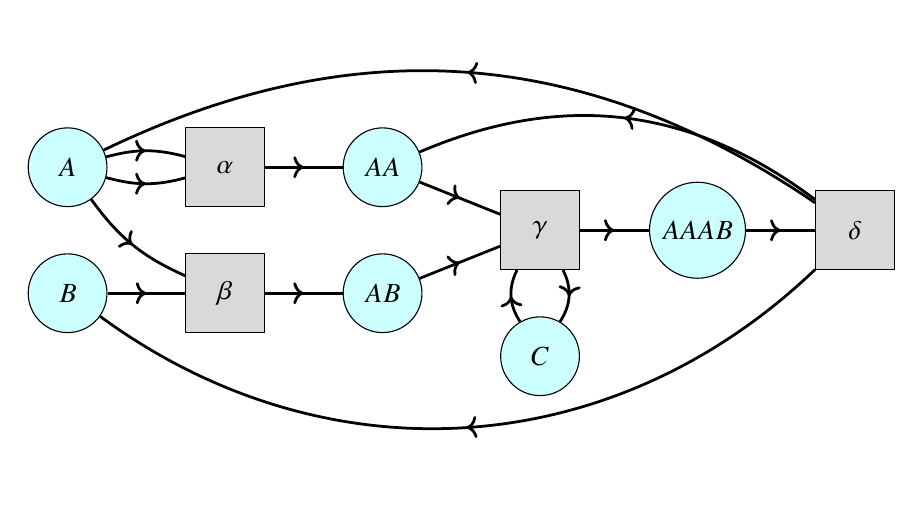
\begin{tikzpicture}
            \begin{pgfonlayer}{nodelayer}
                \node [style=site] (A) at (0, 0.8) {$A$};
                \node [style=site] (B) at (0, -0.8) {$B$};
                \node [style=site] (C) at (6, -1.6) {$C$};
                \node [style=site] (AA) at (4, 0.8) {$AA$};
                \node [style=site] (AB) at (4, -0.8) {$AB$};
                \node [style=site] (AAAB) at (8, 0) {$AAAB$};
                \node [style=transition] (tau1) at (2, 0.8) {$\alpha$};
                \node [style=transition] (tau2) at (2, -0.8) {$\beta$};
                \node [style=transition] (tau3) at (6, 0) {$\gamma$};
                \node [style=transition] (tau4) at (10, 0) {$\delta$};
            \end{pgfonlayer}
            \begin{pgfonlayer}{edgelayer}
                \draw [style=arrow, bend right=15] (A) to (tau1);
                \draw [style=arrow, bend left=15] (A) to (tau1);
                \draw [style=arrow, bend right=15] (A) to (tau2);
                \draw [style=arrow] (tau1) to (AA);
                \draw [style=arrow] (B) to (tau2);
                \draw [style=arrow] (tau2) to (AB);
                \draw [style=arrow] (AA) to (tau3);
                \draw [style=arrow] (AB) to (tau3);
                \draw [style=arrow, bend left=30] (C) to (tau3);
                \draw [style=arrow] (tau3) to (AAAB);
                \draw [style=arrow, bend left=30] (tau3) to (C);
                \draw [style=arrow] (AAAB) to (tau4);
                \draw [style=arrow, bend right=30] (tau4) to (A);
                \draw [style=arrow, bend right=30] (tau4) to (AA);
                \draw [style=arrow, bend left=40] (tau4) to (B);
            \end{pgfonlayer}
        \end{tikzpicture}
    }
\end{center}

This particular example exhibits a number of interesting features.
First, there are transitions wherein one of the input sites is also an output site, namely $\gamma$'s dependence on $C$.
Drawing from chemical parlance, this represents a catalytic effect; the transition can only proceed when the site is present\footnote{The addition of another transitition next to $\gamma$ which does not depend on or yield $C$ can model a process that can proceed without $C$ but is accelerated by it's presence.}.
Second, transitions such as $\delta$ can be viewed as a degradation or disassembly process.
This allows reactions to run in both directions.
To elaborate on this point, we can return to the water example and introduce a second transition allowing for the degradation of water back into diatomic Hydrogen and diatomic Oxygen:

\begin{center}
    \scalebox{0.6}{
        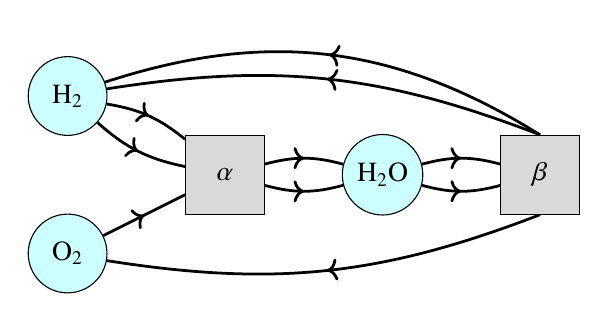
\begin{tikzpicture}
            \begin{pgfonlayer}{nodelayer}
                \node [style=site] (H2) at (0, 1) {$\ce{H_2}$};
                \node [style=site] (O2) at (0, -1) {$\ce{O_2}$};
                \node [style=site] (H2O) at (4, 0) {$\ce{H_2O}$};
                \node [style=transition] (alpha) at (2, 0) {$\alpha$};
                \node [style=transition] (beta) at (6, 0) {$\beta$};
            \end{pgfonlayer}
            \begin{pgfonlayer}{edgelayer}
                \draw [style=arrow, bend right=15] (H2) to (alpha);
                \draw [style=arrow, bend left=15] (H2) to (alpha);
                \draw [style=arrow] (O2) to (alpha);
                \draw [style=arrow, bend right=15] (alpha) to (H2O);
                \draw [style=arrow, bend left=15] (alpha) to (H2O);
                \draw [style=arrow, bend right=15] (H2O) to (beta);
                \draw [style=arrow, bend left=15] (H2O) to (beta);
                \draw [style=arrow, bend right=25] (beta.north) to (H2);
                \draw [style=arrow, bend right=15] (beta.north) to (H2);
                \draw [style=arrow, bend left=15] (beta.south) to (O2);
            \end{pgfonlayer}
        \end{tikzpicture}
    }
\end{center}

An element of $\N[S(P)]$ is called a \textbf{marking} of the Petri net.
Markings play an important role in modeling dynamical systems with Petri nets, representing the state of the system at some time.
For example, the linear combination $5\ce{H_2} + 2\ce{O_2}$ might be thought to represent a system with $5$ molecules of $\ce{H_2}$ and $2$ molecules of $\ce{O_2}$ and no $\ce{H_2O}$.
From this element, we can see that, at least in principle, the transition $\alpha$ might be carried out at most twice\footnote{This is assuming no water dissociates after formation}.
The question of whether, under the action of some dynamical model, one marking can be transformed or processed into another is referred to as the reachability problem and is remarkably difficult.
While we will not delve into dynamical aspects of Petri nets or the to-be-defined assembly spaces in this work, dynamics will likely be a key element of the formal theory going forward.

It is natural, once a mathematical structure has been defined, to ask how two instantiations of that structure may be mapped to one another.
There is, of course, a well defined notion of a map between Petri nets, termed here a \textit{Petri net morphism}, which maps sites and transitions of one Petri net into another in a way that is compatible and consistent with the source and target maps of both Petri nets.
These Petri net morphisms will play a crucial roll in the establishment of bounds for the assembly index in \Cref{sec:assembly-index-bounds}.

\begin{definition}\label{def:petri-map}
    A \textbf{Petri net morphism} from a Petri net $P$ to a Petri net $Q$, denoted $f : P \rightarrow Q$, consisists of a pair of functions $T(f) : T(P) \rightarrow T(Q)$ and $S(f): S(P) \rightarrow S(Q))$ such that the following diagrams commute:
    \begin{equation*}
        \begin{tikzcd}
            T(P)
            \arrow[r, "\sigma_P"]
            \arrow[d, "T(f)", swap]
            &
            \N[S(P)]
            \arrow[d, "\N \lbrack S(f) \rbrack"]
            \\
            T(Q)
            \arrow[r, "\sigma_Q"]
            &
            \N[S(Q)]
        \end{tikzcd}
        \quad
        \textrm{and}
        \quad
        \begin{tikzcd}
            T(P)
            \arrow[r, "\tau_P"]
            \arrow[d, "T(f)", swap]
            &
            \N[S(P)]
            \arrow[d, "\N \lbrack S(f) \rbrack"]
            \\
            T(Q)
            \arrow[r, "\tau_Q"]
            &
            \N[S(Q)].
        \end{tikzcd}
    \end{equation*}
    When possible, we will abuse notation and write $f(s)$ or $f(t)$ for sites $s \in S(P)$ and transitions $t \in T(P)$, in lieu of the more verbose $S(f)(s)$ and $T(f)(t)$.
\end{definition}

The commutative diagrams in this definition are what we mean by ``compatible and consistent".
They essentially encode the idea that asking for a transition's inputs/outputs and then mapping those inputs/outputs into the new Petri network will give you the same result as first mapping the transition and then asking for the inputs/outputs of the image.
To clarify this point, consider the two Petri nets $P$ and $Q$

\begin{center}
    \scalebox{0.6}{
        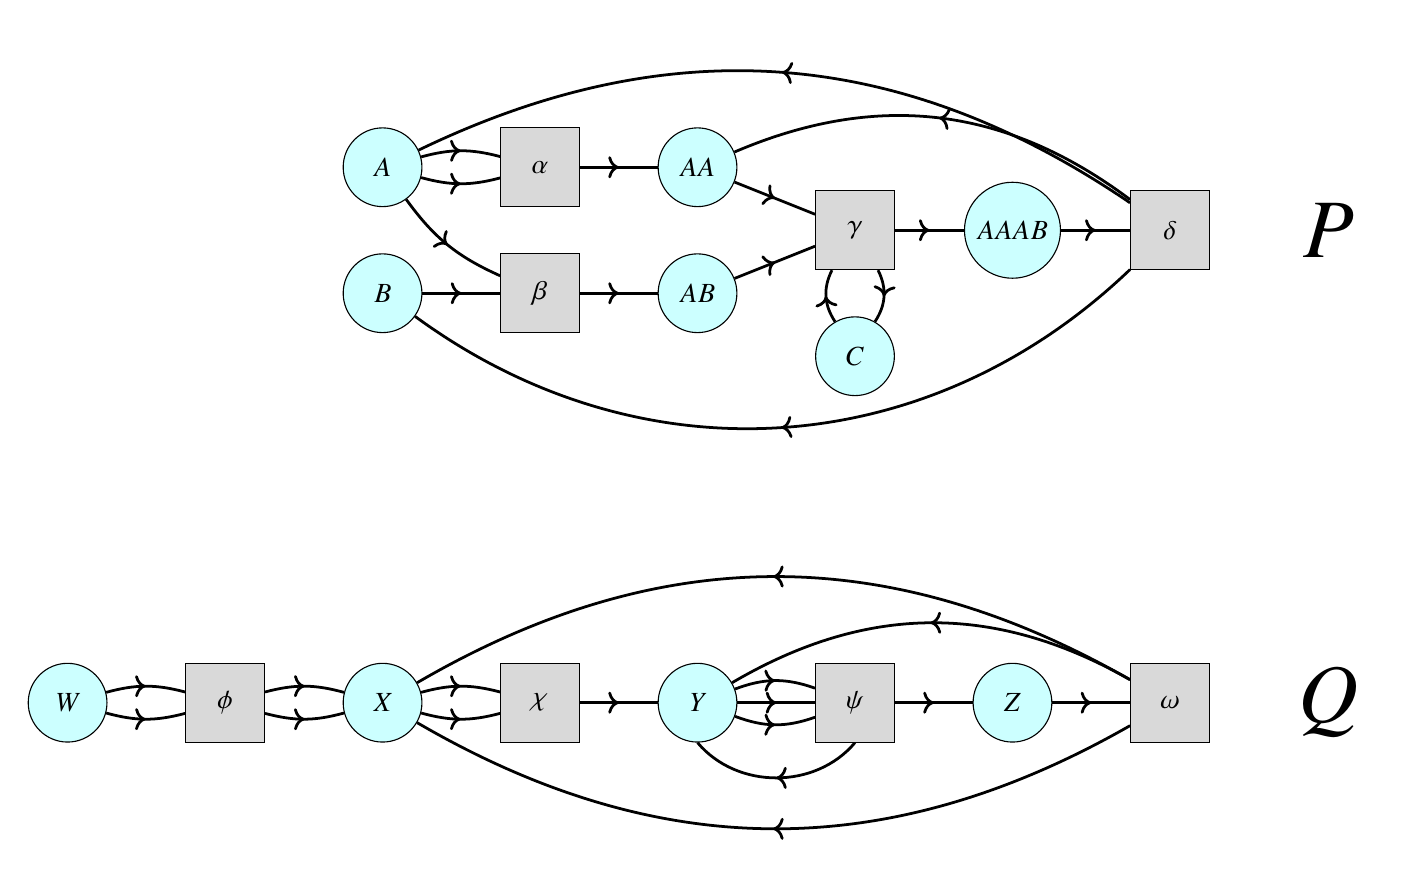
\begin{tikzpicture}
            \begin{pgfonlayer}{nodelayer}
                \node [scale=3] (P) at (12, 0) {$P$};
                \node [style=site] (A) at (0, 0.8) {$A$};
                \node [style=site] (B) at (0, -0.8) {$B$};
                \node [style=site] (C) at (6, -1.6) {$C$};
                \node [style=site] (AA) at (4, 0.8) {$AA$};
                \node [style=site] (AB) at (4, -0.8) {$AB$};
                \node [style=site] (AAAB) at (8, 0) {$AAAB$};
                \node [style=transition] (tau1) at (2, 0.8) {$\alpha$};
                \node [style=transition] (tau2) at (2, -0.8) {$\beta$};
                \node [style=transition] (tau3) at (6, 0) {$\gamma$};
                \node [style=transition] (tau4) at (10, 0) {$\delta$};

                \node [scale=3] (Q) at (12, -6) {$Q$};
                \node [style=site] (W) at (-4, -6) {$W$};
                \node [style=site] (X) at (0, -6) {$X$};
                \node [style=site] (Y) at (4, -6) {$Y$};
                \node [style=site] (Z) at (8, -6) {$Z$};
                \node [style=transition] (tau5) at (-2, -6) {$\phi$};
                \node [style=transition] (tau6) at (2, -6) {$\chi$};
                \node [style=transition] (tau7) at (6, -6) {$\psi$};
                \node [style=transition] (tau8) at (10, -6) {$\omega$};
            \end{pgfonlayer}
            \begin{pgfonlayer}{edgelayer}
                \draw [style=arrow, bend right=15] (A) to (tau1);
                \draw [style=arrow, bend left=15] (A) to (tau1);
                \draw [style=arrow, bend right=15] (A) to (tau2);
                \draw [style=arrow] (tau1) to (AA);
                \draw [style=arrow] (B) to (tau2);
                \draw [style=arrow] (tau2) to (AB);
                \draw [style=arrow] (AA) to (tau3);
                \draw [style=arrow] (AB) to (tau3);
                \draw [style=arrow, bend left=30] (C) to (tau3);
                \draw [style=arrow] (tau3) to (AAAB);
                \draw [style=arrow, bend left=30] (tau3) to (C);
                \draw [style=arrow] (AAAB) to (tau4);
                \draw [style=arrow, bend right=30] (tau4) to (A);
                \draw [style=arrow, bend right=30] (tau4) to (AA);
                \draw [style=arrow, bend left=40] (tau4) to (B);

                \draw [style=arrow, bend left=15] (W) to (tau5);
                \draw [style=arrow, bend right=15] (W) to (tau5);
                \draw [style=arrow, bend left=15] (tau5) to (X);
                \draw [style=arrow, bend right=15] (tau5) to (X);
                \draw [style=arrow, bend left=15] (X) to (tau6);
                \draw [style=arrow, bend right=15] (X) to (tau6);
                \draw [style=arrow] (tau6) to (Y);
                \draw [style=arrow, bend left=20] (Y) to (tau7);
                \draw [style=arrow] (Y) to (tau7);
                \draw [style=arrow, bend right=20] (Y) to (tau7);
                \draw [style=arrow] (tau7) to (Z);
                \draw [style=arrow, bend left=50] (tau7.south) to (Y.south);
                \draw [style=arrow] (Z) to (tau8);
                \draw [style=arrow, bend left=30] (tau8) to (X);
                \draw [style=arrow, bend right=30] (tau8) to (X);
                \draw [style=arrow, bend right=30] (tau8) to (Y);
            \end{pgfonlayer}
        \end{tikzpicture}
    }
\end{center}

We can construct Petri net morphism $f: P \rightarrow Q$ such that
\begin{align*}
    S(f)(\alpha) &= S(f)(\beta) = \chi    & T(f)&(A)    = T(f)(B) = X \\
    S(f)(\gamma) &= \psi                  & T(f)&(AA)   = T(f)(AB) = T(f)(C) = Y \\
    S(f)(\delta) &= \omega                & T(f)&(AAAB) = Z.
\end{align*}

Graphically, this might be depicted as two sets of arrows $T(f)$ and $S(f)$ which map transitions to transitions and sites to sites, respectively colored blue and red.
\begin{center}
    \scalebox{0.6}{
        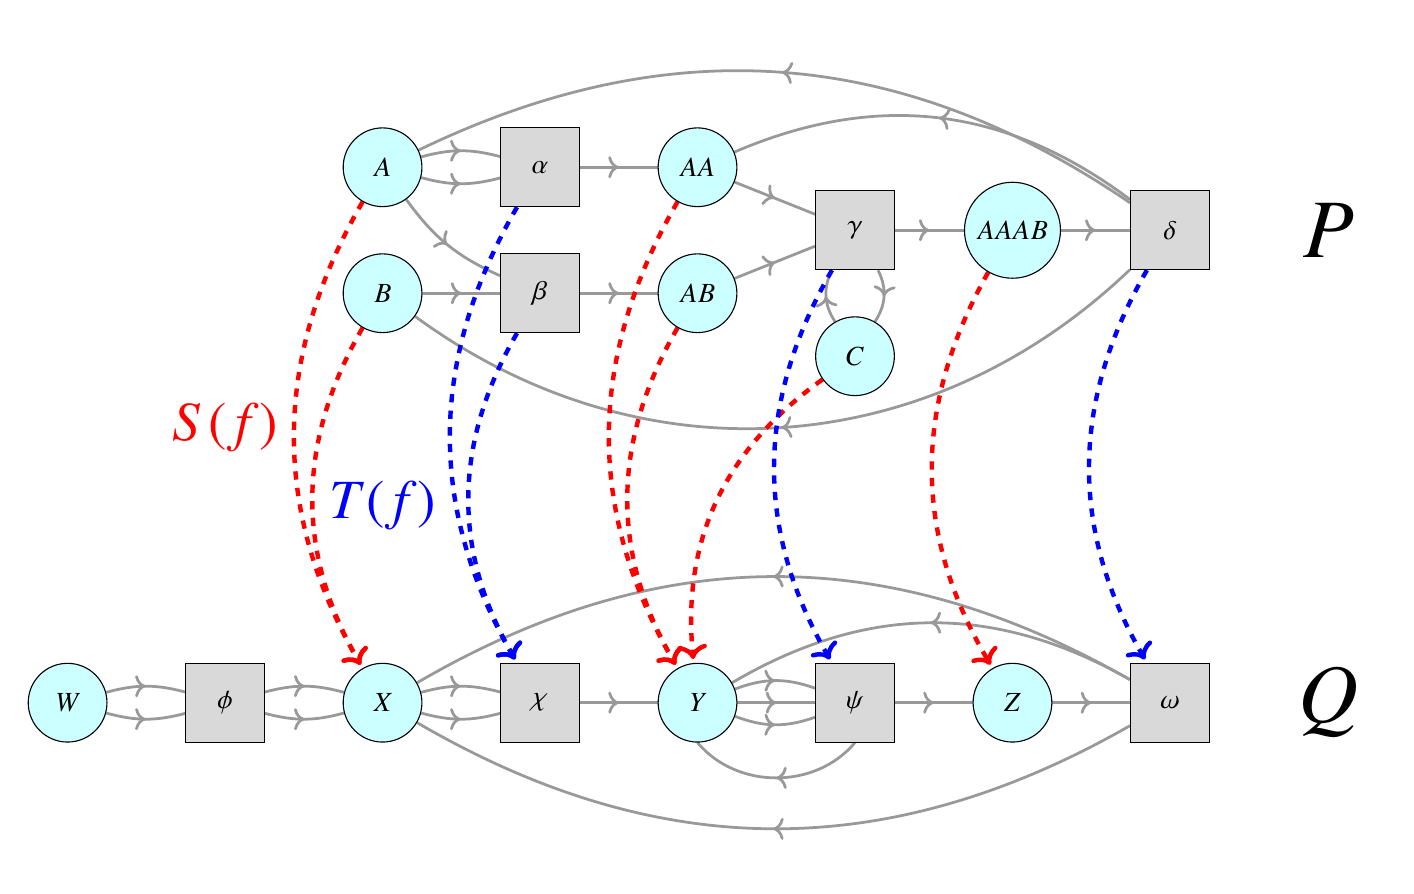
\begin{tikzpicture}
            \begin{pgfonlayer}{nodelayer}
                \node [scale=3] (P) at (12, 0) {$P$};
                \node [style=site] (A) at (0, 0.8) {$A$};
                \node [style=site] (B) at (0, -0.8) {$B$};
                \node [style=site] (C) at (6, -1.6) {$C$};
                \node [style=site] (AA) at (4, 0.8) {$AA$};
                \node [style=site] (AB) at (4, -0.8) {$AB$};
                \node [style=site] (AAAB) at (8, 0) {$AAAB$};
                \node [style=transition] (tau1) at (2, 0.8) {$\alpha$};
                \node [style=transition] (tau2) at (2, -0.8) {$\beta$};
                \node [style=transition] (tau3) at (6, 0) {$\gamma$};
                \node [style=transition] (tau4) at (10, 0) {$\delta$};

                \node [scale=3] (Q) at (12, -6) {$Q$};
                \node [style=site] (W) at (-4, -6) {$W$};
                \node [style=site] (X) at (0, -6) {$X$};
                \node [style=site] (Y) at (4, -6) {$Y$};
                \node [style=site] (Z) at (8, -6) {$Z$};
                \node [style=transition] (tau5) at (-2, -6) {$\phi$};
                \node [style=transition] (tau6) at (2, -6) {$\chi$};
                \node [style=transition] (tau7) at (6, -6) {$\psi$};
                \node [style=transition] (tau8) at (10, -6) {$\omega$};

                \node [text=red, scale=2] (s) at (-2, -2.5) {$S(f)$};
                \node [text=blue, scale=2] (t) at (0, -3.5) {$T(f)$};
            \end{pgfonlayer}
            \begin{pgfonlayer}{edgelayer}
                \draw [style=arrow, draw=gray!80, bend right=15] (A) to (tau1);
                \draw [style=arrow, draw=gray!80, bend left=15] (A) to (tau1);
                \draw [style=arrow, draw=gray!80, bend right=15] (A) to (tau2);
                \draw [style=arrow, draw=gray!80] (tau1) to (AA);
                \draw [style=arrow, draw=gray!80] (B) to (tau2);
                \draw [style=arrow, draw=gray!80] (tau2) to (AB);
                \draw [style=arrow, draw=gray!80] (AA) to (tau3);
                \draw [style=arrow, draw=gray!80] (AB) to (tau3);
                \draw [style=arrow, draw=gray!80, bend left=30] (C) to (tau3);
                \draw [style=arrow, draw=gray!80] (tau3) to (AAAB);
                \draw [style=arrow, draw=gray!80, bend left=30] (tau3) to (C);
                \draw [style=arrow, draw=gray!80] (AAAB) to (tau4);
                \draw [style=arrow, draw=gray!80, bend right=30] (tau4) to (A);
                \draw [style=arrow, draw=gray!80, bend right=30] (tau4) to (AA);
                \draw [style=arrow, draw=gray!80, bend left=40] (tau4) to (B);

                \draw [style=arrow, draw=gray!80, bend left=15] (W) to (tau5);
                \draw [style=arrow, draw=gray!80, bend right=15] (W) to (tau5);
                \draw [style=arrow, draw=gray!80, bend left=15] (tau5) to (X);
                \draw [style=arrow, draw=gray!80, bend right=15] (tau5) to (X);
                \draw [style=arrow, draw=gray!80, bend left=15] (X) to (tau6);
                \draw [style=arrow, draw=gray!80, bend right=15] (X) to (tau6);
                \draw [style=arrow, draw=gray!80] (tau6) to (Y);
                \draw [style=arrow, draw=gray!80, bend left=20] (Y) to (tau7);
                \draw [style=arrow, draw=gray!80] (Y) to (tau7);
                \draw [style=arrow, draw=gray!80, bend right=20] (Y) to (tau7);
                \draw [style=arrow, draw=gray!80] (tau7) to (Z);
                \draw [style=arrow, draw=gray!80, bend left=50] (tau7.south) to (Y.south);
                \draw [style=arrow, draw=gray!80] (Z) to (tau8);
                \draw [style=arrow, draw=gray!80, bend left=30] (tau8) to (X);
                \draw [style=arrow, draw=gray!80, bend right=30] (tau8) to (X);
                \draw [style=arrow, draw=gray!80, bend right=30] (tau8) to (Y);

                \draw [style=sitemap, bend right=30] (A) to (X);
                \draw [style=sitemap, bend right=30] (B) to (X);
                \draw [style=sitemap, bend right=30] (AA) to (Y);
                \draw [style=sitemap, bend right=30] (AB) to (Y);
                \draw [style=sitemap, bend right=30] (C) to (Y);
                \draw [style=sitemap, bend right=30] (AAAB) to (Z);
                \draw [style=transitionmap, bend right=30] (tau1) to (tau6);
                \draw [style=transitionmap, bend right=30] (tau2) to (tau6);
                \draw [style=transitionmap, bend right=30] (tau3) to (tau7);
                \draw [style=transitionmap, bend right=30] (tau4) to (tau8);
            \end{pgfonlayer}
        \end{tikzpicture}
    }
\end{center}

It is easy to see by inspection that $f$ makes the diagrams in \cref{def:petri-map} commute; for example,
\begin{equation*}
    \sigma_Q(T(f)(\alpha)) = 2X = \N[S(f)](\sigma_P(\alpha)).
\end{equation*}

With an understanding of how to map Petri nets to one another, we can now turn to structural properties and relationships, starting with the concept of a subnet.
In essense, a Petri subnet is simply a Petri net whose sets of sites and transitions are subsets of another net and whose source and target maps are compatible.

\begin{definition}\label{def:subnet}
    Let $Q$ be a Petri net. A \textbf{Petri subnet} $P$ of $Q$ consists of
    \begin{itemize}
        \item a subset of sites of $Q$, denoted $S(P)$
        \item a subset of transitions of $Q$, denoted $T(P)$
        \item a pair of maps $\begin{tikzcd}
                T(P)
                \arrow[r, shift left = 1, "\sigma_P"]
                \arrow[r, shift right = 1, "\tau_P", swap]
                &
                \N[S(P)]
        \end{tikzcd}$.
    \end{itemize}
    such that $\sigma_P = \sigma_Q|_{T(P)}$ and $\tau_P = \tau_Q|_{T(P)}$.
    We denote this relationship as $P \subseteq Q$.
\end{definition}

For example, each of the following nets are Petri subnets of our ligation net:
\begin{center}
    \scalebox{0.6}{
        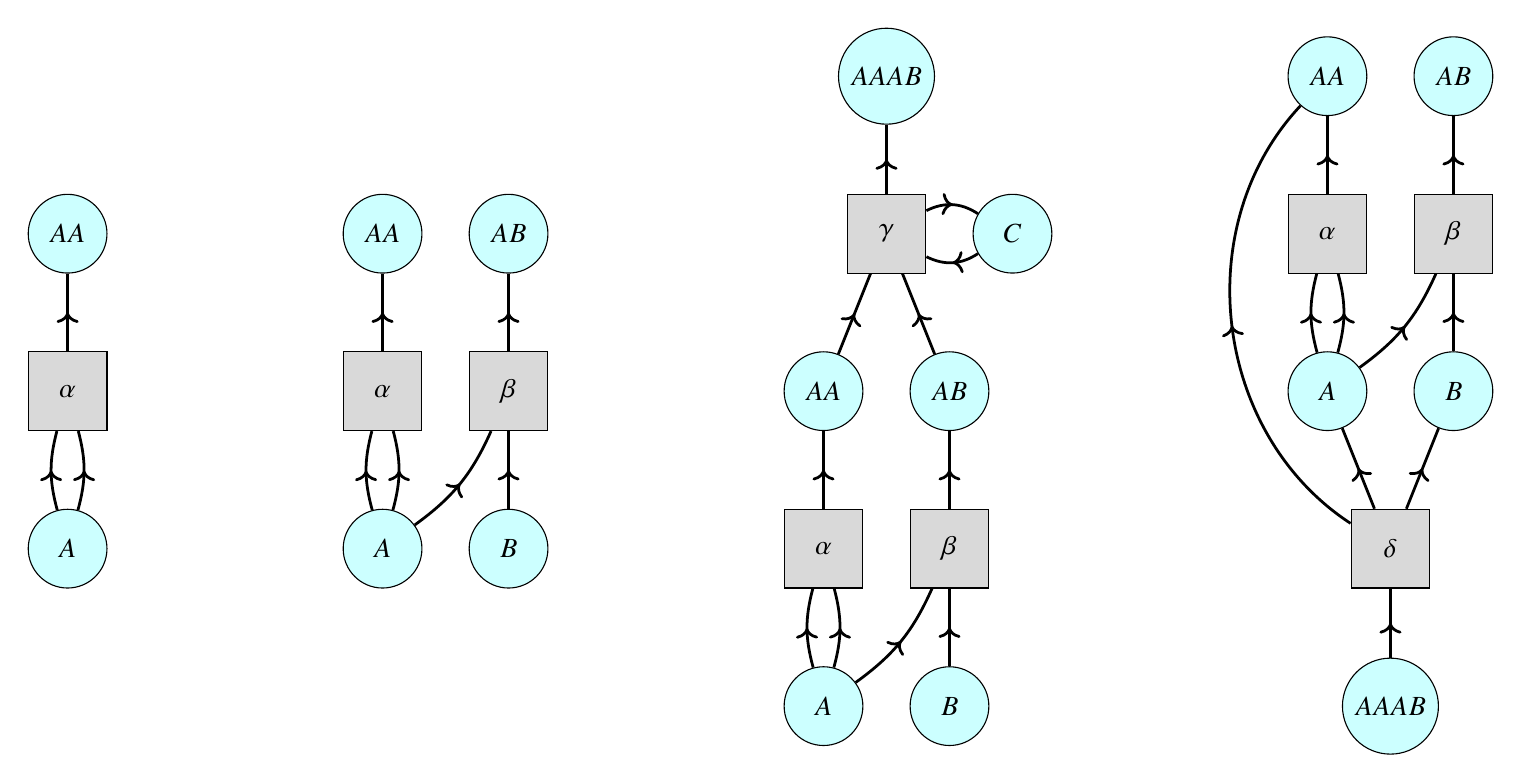
\begin{tikzpicture}
            \begin{pgfonlayer}{nodelayer}
                \node [style=site] (A1) at (0, 2) {$A$};
                \node [style=site] (AA1) at (0, 6) {$AA$};
                \node [style=transition] (tau11) at (0, 4) {$\alpha$};

                \node [style=site] (A2) at (4, 2) {$A$};
                \node [style=site] (B2) at (5.6, 2) {$B$};
                \node [style=site] (AA2) at (4, 6) {$AA$};
                \node [style=site] (AB2) at (5.6, 6) {$AB$};
                \node [style=transition] (tau12) at (4, 4) {$\alpha$};
                \node [style=transition] (tau22) at (5.6, 4) {$\beta$};

                \node [style=site] (A3) at (9.6, 0) {$A$};
                \node [style=site] (B3) at (11.2, 0) {$B$};
                \node [style=site] (C3) at (12, 6) {$C$};
                \node [style=site] (AA3) at (9.6, 4) {$AA$};
                \node [style=site] (AB3) at (11.2, 4) {$AB$};
                \node [style=site] (AAAB3) at (10.4, 8) {$AAAB$};
                \node [style=transition] (tau13) at (9.6, 2) {$\alpha$};
                \node [style=transition] (tau23) at (11.2, 2) {$\beta$};
                \node [style=transition] (tau33) at (10.4, 6) {$\gamma$};

                \node [style=site] (AAAB4) at (16.8, 0) {$AAAB$};
                \node [style=site] (A4) at (16, 4) {$A$};
                \node [style=site] (B4) at (17.6, 4) {$B$};
                \node [style=site] (AA4) at (16, 8) {$AA$};
                \node [style=site] (AB4) at (17.6, 8) {$AB$};
                \node [style=transition] (tau44) at (16.8, 2) {$\delta$};
                \node [style=transition] (tau14) at (16, 6) {$\alpha$};
                \node [style=transition] (tau24) at (17.6, 6) {$\beta$};
            \end{pgfonlayer}
            \begin{pgfonlayer}{edgelayer}
                \draw [style=arrow, bend right=15] (A1) to (tau11);
                \draw [style=arrow, bend left=15] (A1) to (tau11);
                \draw [style=arrow] (tau11) to (AA1);

                \draw [style=arrow, bend right=15] (A2) to (tau12);
                \draw [style=arrow, bend left=15] (A2) to (tau12);
                \draw [style=arrow, bend right=15] (A2) to (tau22);
                \draw [style=arrow] (B2) to (tau22);
                \draw [style=arrow] (tau12) to (AA2);
                \draw [style=arrow] (tau22) to (AB2);

                \draw [style=arrow, bend right=15] (A3) to (tau13);
                \draw [style=arrow, bend left=15] (A3) to (tau13);
                \draw [style=arrow, bend right=15] (A3) to (tau23);
                \draw [style=arrow] (tau13) to (AA3);
                \draw [style=arrow] (B3) to (tau23);
                \draw [style=arrow] (tau23) to (AB3);
                \draw [style=arrow] (AA3) to (tau33);
                \draw [style=arrow] (AB3) to (tau33);
                \draw [style=arrow, bend left=30] (C3) to (tau33);
                \draw [style=arrow] (tau33) to (AAAB3);
                \draw [style=arrow, bend left=30] (tau33) to (C3);

                \draw [style=arrow] (AAAB4) to (tau44);
                \draw [style=arrow] (tau44) to (A4);
                \draw [style=arrow, bend left=50] (tau44) to (AA4);
                \draw [style=arrow] (tau44) to (B4);
                \draw [style=arrow, bend left=15] (A4) to (tau14);
                \draw [style=arrow, bend right=15] (A4) to (tau14);
                \draw [style=arrow, bend right=15] (A4) to (tau24);
                \draw [style=arrow] (B4) to (tau24);
                \draw [style=arrow] (tau14) to (AA4);
                \draw [style=arrow] (tau24) to (AB4);
            \end{pgfonlayer}
        \end{tikzpicture}
    }
\end{center}

\begin{definition}
    Let $P$ be a Petri net and let $Q \subseteq P$.
    We say that $Q$ \textit{spans} $P$ if $S(Q) = S(P)$.
    \TODO{New Definition. Integrate with surrounding text.}
\end{definition}

Petri net morphisms and subnets interact well.
In particular, for a Petri net morphism $f : P \rightarrow Q$, the image $f(P)$ in $Q$ is a Petri subnet with source and target maps $\sigma_{f(P)}$ and $\tau_{f(P)}$ defined by restriction of $\sigma_Q$ and $\tau_Q$, respectively.
Similarly, the preimage of a Petri subnet of $Q$ is a Petri subnet of $P$ with source and target maps defined by restriction of $\sigma_P$ and $\tau_P$.
Continuing the example map from our ligation model,
\begin{center}
    \scalebox{0.6}{
        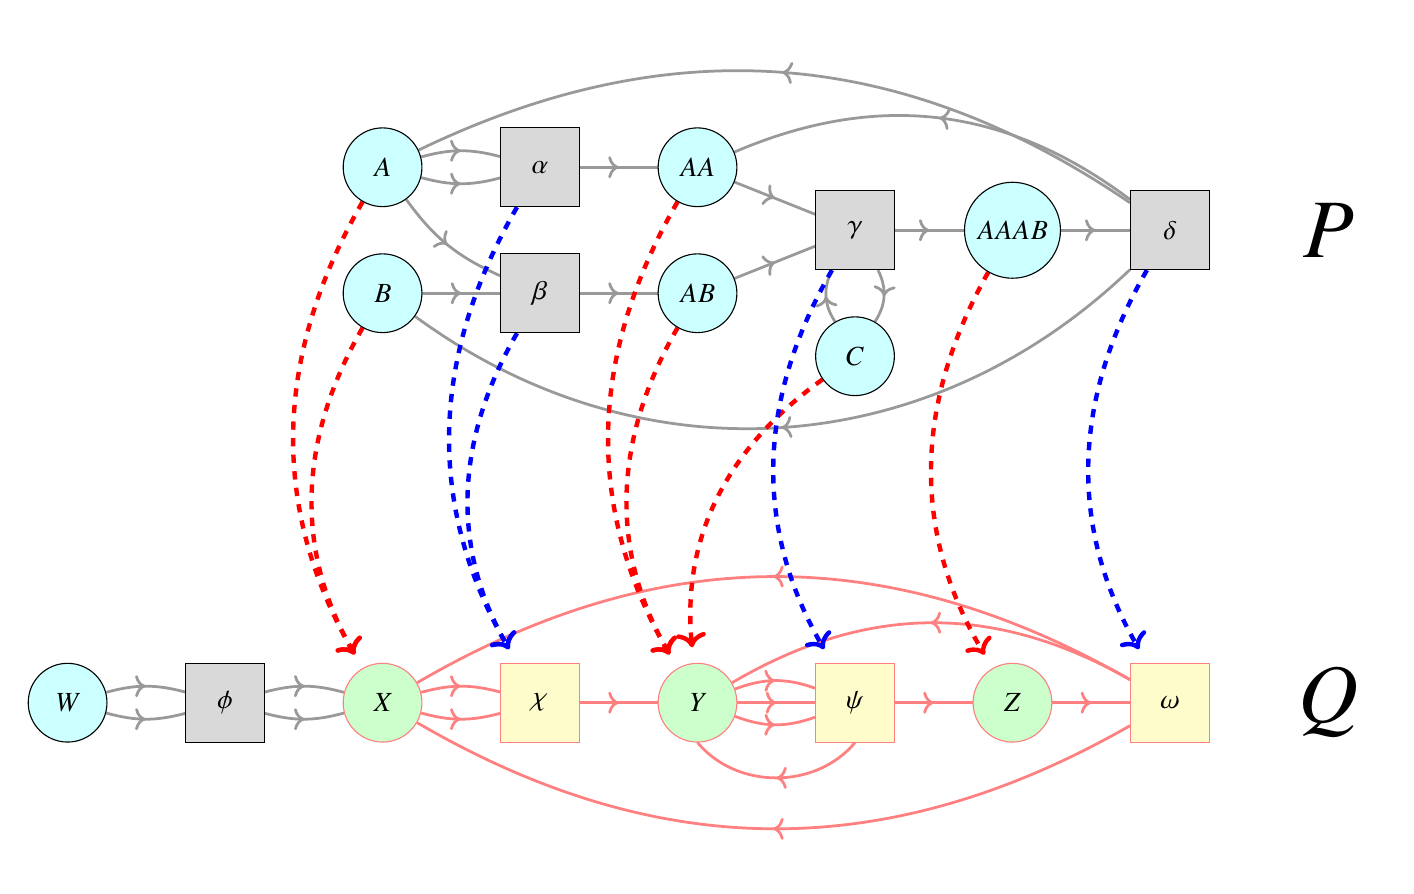
\begin{tikzpicture}
            \begin{pgfonlayer}{nodelayer}
                \node [scale=3] (P) at (12, 0) {$P$};
                \node [style=site] (A) at (0, 0.8) {$A$};
                \node [style=site] (B) at (0, -0.8) {$B$};
                \node [style=site] (C) at (6, -1.6) {$C$};
                \node [style=site] (AA) at (4, 0.8) {$AA$};
                \node [style=site] (AB) at (4, -0.8) {$AB$};
                \node [style=site] (AAAB) at (8, 0) {$AAAB$};
                \node [style=transition] (tau1) at (2, 0.8) {$\alpha$};
                \node [style=transition] (tau2) at (2, -0.8) {$\beta$};
                \node [style=transition] (tau3) at (6, 0) {$\gamma$};
                \node [style=transition] (tau4) at (10, 0) {$\delta$};

                \node [scale=3] (Q) at (12, -6) {$Q$};
                \node [style=site] (W) at (-4, -6) {$W$};
                \node [style=site, fill=green!20, draw=red!50] (X) at (0, -6) {$X$};
                \node [style=site, fill=green!20, draw=red!50] (Y) at (4, -6) {$Y$};
                \node [style=site, fill=green!20, draw=red!50] (Z) at (8, -6) {$Z$};
                \node [style=transition] (tau5) at (-2, -6) {$\phi$};
                \node [style=transition, fill=yellow!20, draw=red!50] (tau6) at (2, -6) {$\chi$};
                \node [style=transition, fill=yellow!20, draw=red!50] (tau7) at (6, -6) {$\psi$};
                \node [style=transition, fill=yellow!20, draw=red!50] (tau8) at (10, -6) {$\omega$};
            \end{pgfonlayer}
            \begin{pgfonlayer}{edgelayer}
                \draw [style=arrow, draw=gray!80, bend right=15] (A) to (tau1);
                \draw [style=arrow, draw=gray!80, bend left=15] (A) to (tau1);
                \draw [style=arrow, draw=gray!80, bend right=15] (A) to (tau2);
                \draw [style=arrow, draw=gray!80] (tau1) to (AA);
                \draw [style=arrow, draw=gray!80] (B) to (tau2);
                \draw [style=arrow, draw=gray!80] (tau2) to (AB);
                \draw [style=arrow, draw=gray!80] (AA) to (tau3);
                \draw [style=arrow, draw=gray!80] (AB) to (tau3);
                \draw [style=arrow, draw=gray!80, bend left=30] (C) to (tau3);
                \draw [style=arrow, draw=gray!80] (tau3) to (AAAB);
                \draw [style=arrow, draw=gray!80, bend left=30] (tau3) to (C);
                \draw [style=arrow, draw=gray!80] (AAAB) to (tau4);
                \draw [style=arrow, draw=gray!80, bend right=30] (tau4) to (A);
                \draw [style=arrow, draw=gray!80, bend right=30] (tau4) to (AA);
                \draw [style=arrow, draw=gray!80, bend left=40] (tau4) to (B);

                \draw [style=arrow, draw=gray!80, bend left=15] (W) to (tau5);
                \draw [style=arrow, draw=gray!80, bend right=15] (W) to (tau5);
                \draw [style=arrow, draw=gray!80, bend left=15] (tau5) to (X);
                \draw [style=arrow, draw=gray!80, bend right=15] (tau5) to (X);
                \draw [style=arrow, draw=red!50, bend left=15] (X) to (tau6);
                \draw [style=arrow, draw=red!50, bend right=15] (X) to (tau6);
                \draw [style=arrow, draw=red!50] (tau6) to (Y);
                \draw [style=arrow, draw=red!50, bend left=20] (Y) to (tau7);
                \draw [style=arrow, draw=red!50] (Y) to (tau7);
                \draw [style=arrow, draw=red!50, bend right=20] (Y) to (tau7);
                \draw [style=arrow, draw=red!50] (tau7) to (Z);
                \draw [style=arrow, draw=red!50, bend left=50] (tau7.south) to (Y.south);
                \draw [style=arrow, draw=red!50] (Z) to (tau8);
                \draw [style=arrow, draw=red!50, bend left=30] (tau8) to (X);
                \draw [style=arrow, draw=red!50, bend right=30] (tau8) to (X);
                \draw [style=arrow, draw=red!50, bend right=30] (tau8) to (Y);

                \draw [style=sitemap, bend right=30, shorten >=2mm] (A) to (X);
                \draw [style=sitemap, bend right=30, shorten >=2mm] (B) to (X);
                \draw [style=sitemap, bend right=30, shorten >=2mm] (AA) to (Y);
                \draw [style=sitemap, bend right=30, shorten >=2mm] (AB) to (Y);
                \draw [style=sitemap, bend right=30, shorten >=2mm] (C) to (Y);
                \draw [style=sitemap, bend right=30, shorten >=2mm] (AAAB) to (Z);
                \draw [style=transitionmap, bend right=30, shorten >=2mm] (tau1) to (tau6);
                \draw [style=transitionmap, bend right=30, shorten >=2mm] (tau2) to (tau6);
                \draw [style=transitionmap, bend right=30, shorten >=2mm] (tau3) to (tau7);
                \draw [style=transitionmap, bend right=30, shorten >=2mm] (tau4) to (tau8);
            \end{pgfonlayer}
        \end{tikzpicture}
    }
\end{center}
the image, outlined in light red, is a subnet of $Q$.

When it comes to describing systems like the construction of a string, or the building of a molecule, it is often classically unphysical for objects to be created from nothing or destroyed.
For that reason, we need to be able to identify aspects of a Petri net that might represent exactly such a process: sources and sinks.
\begin{definition}\label{def:source-sink}
    Let $P$ be a Petri net and let $t$ be a transition.
    We say that $t$ is a \textbf{source} if $\sigma(t) = 0$, and is a \textbf{sink} if $\tau(t) = 0$.
    $P$ is said to be \textbf{sourceless} if it has no sources.
    Similarly, $P$ is \textbf{sinkless} if it has no sinks.
\end{definition}

Graphically, 
\begin{center}
    \scalebox{0.6}{
        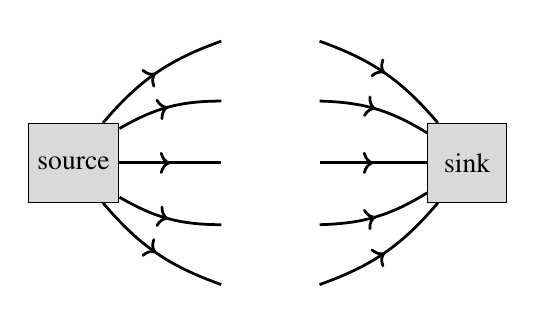
\begin{tikzpicture}
            \begin{pgfonlayer}{nodelayer}
                \node [style=transition] (source) at (0, 0) {source};
                \node (A) at (2, 1.6) {};
                \node (B) at (2, 0.8) {};
                \node (C) at (2, 0) {};
                \node (D) at (2, -0.8) {};
                \node (E) at (2, -1.6) {};

                \node (F) at (3, 1.6) {};
                \node (G) at (3, 0.8) {};
                \node (H) at (3, 0) {};
                \node (I) at (3, -0.8) {};
                \node (J) at (3, -1.6) {};
                \node [style=transition] (sink) at (5, 0) {sink};
            \end{pgfonlayer}
            \begin{pgfonlayer}{edgelayer}
                \draw [style=arrow, bend left=15] (source) to (A);
                \draw [style=arrow, bend left=15] (source) to (B);
                \draw [style=arrow] (source) to (C);
                \draw [style=arrow, bend right=15] (source) to (D);
                \draw [style=arrow, bend right=15] (source) to (E);

                \draw [style=arrow, bend left=15] (F) to (sink);
                \draw [style=arrow, bend left=15] (G) to (sink);
                \draw [style=arrow] (H) to (sink);
                \draw [style=arrow, bend right=15] (I) to (sink);
                \draw [style=arrow, bend right=15] (J) to (sink);
            \end{pgfonlayer}
        \end{tikzpicture}
    }
\end{center}
It follows immediately from the definition of a Petri map that the image of a sourceless Petri net is sourceless, otherwise the $\sigma$-diagram would not commute.
Similarly, the image of a sinkless Petri net is sinkless.

Up to this point, all of the defintions have been fairly standard, at least in terms of concepts.
We now start constructing apparently new ideas that will allow us to formalize the concepts of an assembly space and the assembly index.
The first of these is the idea of a pathway.
Suppose you begin with a set of objects $X$ and wish to consider ways of building some other set of objects.
The simplest approach is to construct a sequence of transitions such that each transition depends only on $X$ or something produced by an earlier transition.
This is what we refer to as a \textit{pathway}.

\begin{definition}\label{def:pathway}
    Let $P$ be a Petri net.
    A \textbf{pathway} in $P$ is a sequence of transitions $\gamma = \pathway{t_n \ldots t_1}$ of length $n \ge 1$ such that for all $1 \le i \le n$
    \begin{equation*}
        \pi(\sigma(t_i)) \subseteq \bigcup_{j=1}^{i-1} \pi(\tau(t_j)).
    \end{equation*}
    We consider the empty sequence of transitions as a pathway and refer to it as the \textbf{zero pathway}.

    \smallskip
    Let $X$ be a subset of sites in $P$. We say that $\gamma$ is \textit{from $X$} if $\pi(\sigma(t_1)) \subseteq X$, and will sometimes say that $\gamma$ starts at $X$.

    \smallskip
    Let $y$ be site, and let $Y$ be a subset of sites.
    We say $\gamma$ is a \textit{to $y$} if $y \in \pi(\tau(t_n))$, and \textit{to $Y$} if $Y \subseteq \pi(\tau(t_n))$, and will sometimes say that $\gamma$ terminates at $y$ or $Y$.

    \smallskip
    We say that the zero pathway is a pathway from any set $X$ to itself and none other.

    \smallskip
    Let $X$ and $Y$ be sets of sites in $P$.
    We say $X$ is \textbf{pathway connected} to $Y$ if there exists a pathway, possibly the zero pathway, from $X$ to $Y$.

    \red{I'd rather express this idea using $\N$ directly instead of using $\pi$}

    \TODO{Break this definition apart}
\end{definition}

Returning to our ligation example, suppose we have the set $X = \{A, B\}$.
There are, in fact, pathways from $X$, counting the zero pathway.
The other three are $\pathway{\alpha}$, $\pathway{\beta}$ and $\pathway{\alpha\beta}$ and $\pathway{\beta\alpha}$.
We depict these pathways below.
The sites in $X$ are outlined in blue, the transitions are filled green, and relevant edges are red.

\begin{center}
    \scalebox{0.6}{
        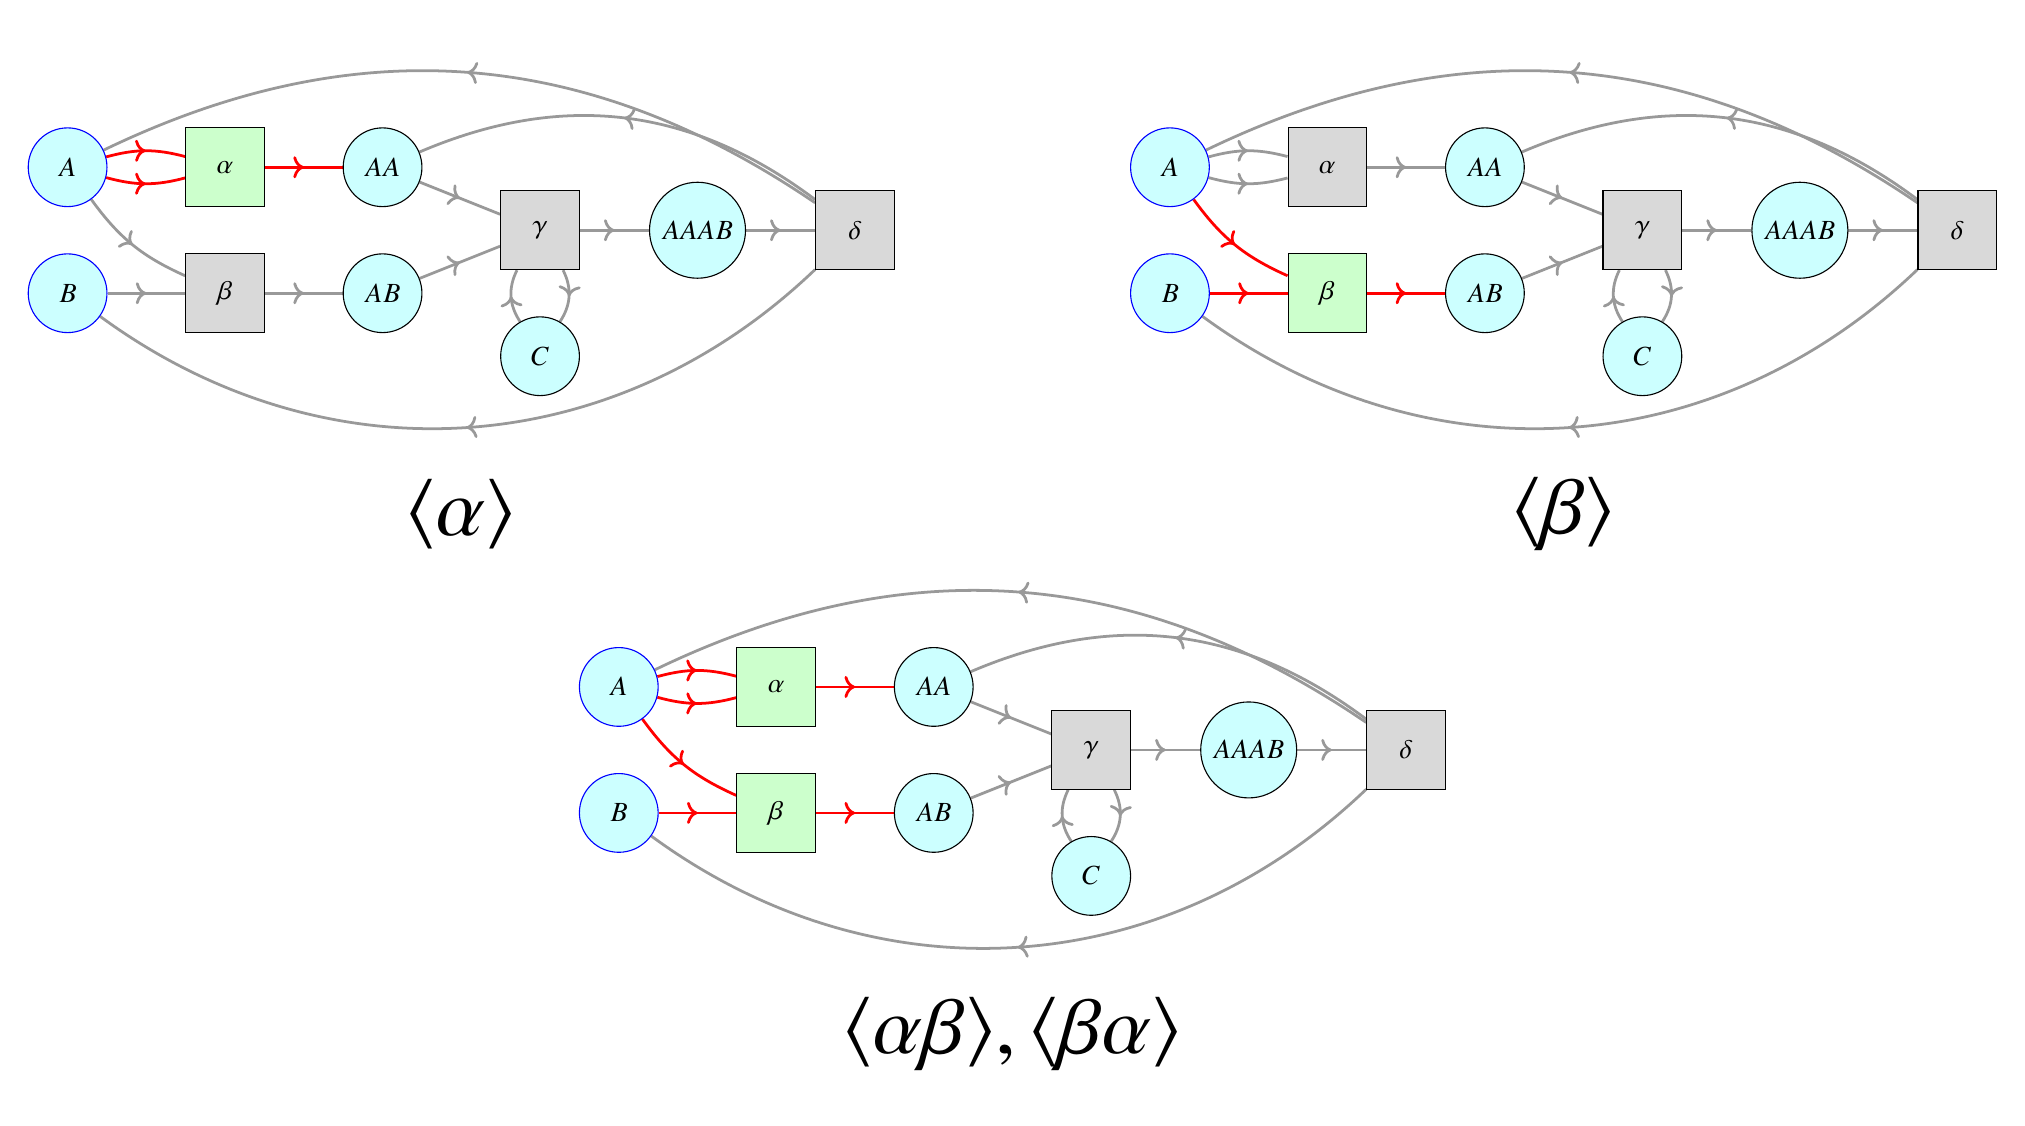
\begin{tikzpicture}
            \begin{pgfonlayer}{nodelayer}
                \node [style=site, draw=blue] (A1) at (0, 0.8) {$A$};
                \node [style=site, draw=blue] (B1) at (0, -0.8) {$B$};
                \node [style=site] (C1) at (6, -1.6) {$C$};
                \node [style=site] (AA1) at (4, 0.8) {$AA$};
                \node [style=site] (AB1) at (4, -0.8) {$AB$};
                \node [style=site] (AAAB1) at (8, 0) {$AAAB$};
                \node [style=transition, fill=green!20] (tau11) at (2, 0.8) {$\alpha$};
                \node [style=transition] (tau21) at (2, -0.8) {$\beta$};
                \node [style=transition] (tau31) at (6, 0) {$\gamma$};
                \node [style=transition] (tau41) at (10, 0) {$\delta$};
                \node [scale=3] at (5, -3.6) {$\pathway{\alpha}$};

                \node [style=site, draw=blue] (A2) at (14, 0.8) {$A$};
                \node [style=site, draw=blue] (B2) at (14, -0.8) {$B$};
                \node [style=site] (C2) at (20, -1.6) {$C$};
                \node [style=site] (AA2) at (18, 0.8) {$AA$};
                \node [style=site] (AB2) at (18, -0.8) {$AB$};
                \node [style=site] (AAAB2) at (22, 0) {$AAAB$};
                \node [style=transition] (tau12) at (16, 0.8) {$\alpha$};
                \node [style=transition, fill=green!20] (tau22) at (16, -0.8) {$\beta$};
                \node [style=transition] (tau32) at (20, 0) {$\gamma$};
                \node [style=transition] (tau42) at (24, 0) {$\delta$};
                \node [scale=3] at (19, -3.6) {$\pathway{\beta}$};

                \node [style=site, draw=blue] (A3) at (7, -5.8) {$A$};
                \node [style=site, draw=blue] (B3) at (7, -7.4) {$B$};
                \node [style=site] (C3) at (13, -8.2) {$C$};
                \node [style=site] (AA3) at (11, -5.8) {$AA$};
                \node [style=site] (AB3) at (11, -7.4) {$AB$};
                \node [style=site] (AAAB3) at (15, -6.6) {$AAAB$};
                \node [style=transition, fill=green!20] (tau13) at (9, -5.8) {$\alpha$};
                \node [style=transition, fill=green!20] (tau23) at (9, -7.4) {$\beta$};
                \node [style=transition] (tau33) at (13, -6.6) {$\gamma$};
                \node [style=transition] (tau43) at (17, -6.6) {$\delta$};
                \node [scale=3] at (12, -10.2) {$\pathway{\alpha\beta}, \pathway{\beta\alpha}$};
            \end{pgfonlayer}
            \begin{pgfonlayer}{edgelayer}
                \draw [style=arrow, draw=red, bend right=15] (A1) to (tau11);
                \draw [style=arrow, draw=red, bend left=15] (A1) to (tau11);
                \draw [style=arrow, draw=gray!80, bend right=15] (A1) to (tau21);
                \draw [style=arrow, draw=red] (tau11) to (AA1);
                \draw [style=arrow, draw=gray!80] (B1) to (tau21);
                \draw [style=arrow, draw=gray!80] (tau21) to (AB1);
                \draw [style=arrow, draw=gray!80] (AA1) to (tau31);
                \draw [style=arrow, draw=gray!80] (AB1) to (tau31);
                \draw [style=arrow, draw=gray!80, bend left=30] (C1) to (tau31);
                \draw [style=arrow, draw=gray!80] (tau31) to (AAAB1);
                \draw [style=arrow, draw=gray!80, bend left=30] (tau31) to (C1);
                \draw [style=arrow, draw=gray!80] (AAAB1) to (tau41);
                \draw [style=arrow, draw=gray!80, bend right=30] (tau41) to (A1);
                \draw [style=arrow, draw=gray!80, bend right=30] (tau41) to (AA1);
                \draw [style=arrow, draw=gray!80, bend left=40] (tau41) to (B1);

                \draw [style=arrow, draw=gray!80, bend right=15] (A2) to (tau12);
                \draw [style=arrow, draw=gray!80, bend left=15] (A2) to (tau12);
                \draw [style=arrow, draw=red, bend right=15] (A2) to (tau22);
                \draw [style=arrow, draw=gray!80] (tau12) to (AA2);
                \draw [style=arrow, draw=red] (B2) to (tau22);
                \draw [style=arrow, draw=red] (tau22) to (AB2);
                \draw [style=arrow, draw=gray!80] (AA2) to (tau32);
                \draw [style=arrow, draw=gray!80] (AB2) to (tau32);
                \draw [style=arrow, draw=gray!80, bend left=30] (C2) to (tau32);
                \draw [style=arrow, draw=gray!80] (tau32) to (AAAB2);
                \draw [style=arrow, draw=gray!80, bend left=30] (tau32) to (C2);
                \draw [style=arrow, draw=gray!80] (AAAB2) to (tau42);
                \draw [style=arrow, draw=gray!80, bend right=30] (tau42) to (A2);
                \draw [style=arrow, draw=gray!80, bend right=30] (tau42) to (AA2);
                \draw [style=arrow, draw=gray!80, bend left=40] (tau42) to (B2);

                \draw [style=arrow, draw=red, bend right=15] (A3) to (tau13);
                \draw [style=arrow, draw=red, bend left=15] (A3) to (tau13);
                \draw [style=arrow, draw=red, bend right=15] (A3) to (tau23);
                \draw [style=arrow, draw=red] (tau13) to (AA3);
                \draw [style=arrow, draw=red] (B3) to (tau23);
                \draw [style=arrow, draw=red] (tau23) to (AB3);
                \draw [style=arrow, draw=gray!80] (AA3) to (tau33);
                \draw [style=arrow, draw=gray!80] (AB3) to (tau33);
                \draw [style=arrow, draw=gray!80, bend left=30] (C3) to (tau33);
                \draw [style=arrow, draw=gray!80] (tau33) to (AAAB3);
                \draw [style=arrow, draw=gray!80, bend left=30] (tau33) to (C3);
                \draw [style=arrow, draw=gray!80] (AAAB3) to (tau43);
                \draw [style=arrow, draw=gray!80, bend right=30] (tau43) to (A3);
                \draw [style=arrow, draw=gray!80, bend right=30] (tau43) to (AA3);
                \draw [style=arrow, draw=gray!80, bend left=40] (tau43) to (B3);
            \end{pgfonlayer}
        \end{tikzpicture}
    }
\end{center}

There are a number of points to make with this example.
First, because we did not include $C$ in our starting set, the pathways cannot include $\gamma$ or consequently $\delta$.
Had $X$ included $C$, there would have been at least one pathway from $X$ to any subset of sites.
This is an important point which we will return to shortly.
Second, the graphical representations of both $\pathway{\alpha\beta}$ and $\pathway{\beta\alpha}$ are identical.
This tells us that the order in which $\alpha$ and $\beta$ fire is unimportant as the result is the same.
Finally, in each case the highlighted sites and transitions form a Petri subnet of the larger net.
In fact, given any set of transitions, we can construct a Petri subnet.

\begin{definition}\label{def:site-completion}
    Let $P$ be a Petri net and let $X$ be a set of transitions in $P$.
    The \textbf{site completion} of $X$, denoted $X^*$ is the Petri subnet of $P$ formed such that
    \begin{itemize}
        \item $T(X^*) = X$
        \item $\displaystyle S(X^*) = \bigcup_{t \in X} \pi(\sigma_P(t) + \tau_P(t))$
        \item $\sigma_{X^*} = \sigma_P|_X$ and $\tau_{X^*} = \tau_P|_X$.
    \end{itemize}
\end{definition}

That the site completion is, in fact, a subnet follows immediately from the definition of a subnet.
Furthermore, since we can view a pathway as an ordered set of transitions, we can simply site complete that set to construct a Petri subnet.
There are several questions we could continue with here, such whether every Petri subnet gives rise to a pathway which uses every transition in the subnet.
However, since questions such as this are immaterial to the problem at hand, we will postpone addressing them to subsequent works.

The value of pathways is that they allow us to consider or construct sets of sites which are sufficient to construct every other object in the space.
We refer to such a subset of objects as a \textit{generating set}.

\begin{definition}\label{def:generating-set}
    Let $P$ be a Petri net and let $X$ be a subset of sites of $P$.
    We say that $X$ is a \textbf{generating set} of $P$ if $X$ is pathway connected to every subset of sites $Y$ in $P$.
    The set of all generating sets of $P$ is denoted $\G_P$.
\end{definition}

To clarify this idea, let us consider a few sets of sites from the ligation example.
The first, and least interesting example, is the set of all sites $\{A, B, AA, AB, C, AAAB\}$.
Clearly every site in the space can be created, or at least provided, from this set.
In fact it is trivially true that for any Petri net $P$, the set of all sites in the net is a generating set, i.e. $\G_P \ne \emptyset$.
Furthermore, the empty set of sites is not generating in this case, though it may be in Petri nets with sources (\Cref{def:source-sink}).
The set $\{A,B\}$ is also not a generating set; what sequence of transitions could yield $C$ or $AAAB$?
It is reassuring to know that not all subsets sites are generating, in this case at least.
However, the set $\{A,B,C\}$ is generating, and we can add any other site to this set and the result will be a generating set, e.g. $\{A,B,C,AAAB\}$.
The sets $\{A, AA, AB, C\}$ and $\{AB, AAAB, C\}$ are generating, but upon close inspection we can see that some of the sites within them are not required, e.g. $A$ or $AA$ in the former, and $AB$ in the latter.
This alludes to the idea of a \textit{minimal} generating set; one from which we can remove no sites and the result still be a generating set.
We can formalize this idea by noting that the set of all generating sets of a Petri net is naturally a subset of the powerset of the sites of the net, $\G_P \subseteq \powerset(S(P))$.
As such, $\G_P$ inherits a partial order from $\powerset(S(P))$ (subset inclusion) within which we can determine if a generating set is minimal.
We refer to a minimal generating set with respect to this partial order as a \textit{basis}.

\begin{definition}\label{def:basis}
    Let $P$ be a Petri net and let $X$ be a generating set of $P$, $X \in \G_P$.
    We say that $X$ is a \textbf{basis} if it is minimal with respect to the set inclusion order on $\G_P$.
\end{definition}

The ligation example admits a choice of basis: $\{A,B,C\}$, $\{A,AB,C\}$, $\{AA,AB,C\}$, or $\{C,AAAB\}$.
While it may seem undesirable, on its face, for a Petri net to admit more than one basis, there is little difference between this and being able to choose the basis of a vector space such as $\R^2$.
We can view each choice of basis as representing a minimal set of starting components from which everything of interest can be constructed; similar to deciding which raw materials to use to build a house, or which chemical reagents to use to synthesis a given set of molecules.
Depending on the context, there may be \textit{a priori} reasons to prefer one basis over another.
For example, in the ligation example, the $\{A,B,C\}$ basis seems somehow preferable as it is composed of monomers while all other bases consist of higher-order components.
To make such a distinction, however, requires additional structure, such as a grading\footnote{Here we use the term \textit{grading} loosely. It could, for example, simply mean a map $g : S(P) \rightarrow \N$ for some Petri net $P$ which is consistent in some way with the graph structure of $P$.} on the sites with which to formally distinguish between bases.
The choice of basis will become important in \Cref{sec:assembly-spaces,sec:assembly-index}, but for now we are only interested in the existence and uniqueness of bases and their preservation under Petri net morphisms.
For this reason, we will leave the question of mechanisms for preferentially choosing a basis for a future work.

Whether or not a Petri net admits a basis at all and whether that basis is unique, are both fundamentally important questions.
The establishment of something like the assembly index of an object relies on the specification of a basis.
Fortuitously, every Petri net admits at least one basis, and in certain cases this basis will be unique.
\begin{lemma}\label{lem:bases-exist}
    Every Petri net admits at least one basis.
\end{lemma}
\begin{proof}
    \TODO{Complete (likely to use Zorn's lemma)}
\end{proof}

If we recall, a generating set (and consequently a basis) is a set of sites from which all others can be reached via a pathway.
However, some objects are priviledged in that there are not pathways which terminate at them.
Consider $C$ in the ligation example:
\begin{center}
    \scalebox{0.6}{
        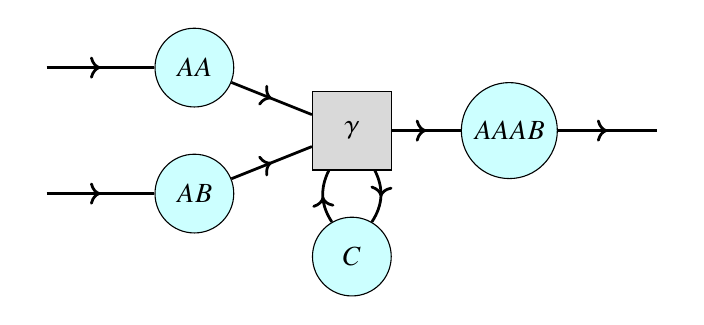
\begin{tikzpicture}
            \begin{pgfonlayer}{nodelayer}
                \node (a) at (-4, 0.8) {};
                \node (b) at (-4, -0.8) {};
                \node (c) at (4, 0) {};
                \node [style=site] (C) at (0, -1.6) {$C$};
                \node [style=site] (AA) at (-2, 0.8) {$AA$};
                \node [style=site] (AB) at (-2, -0.8) {$AB$};
                \node [style=site] (AAAB) at (2, 0) {$AAAB$};
                \node [style=transition] (gamma) at (0, 0) {$\gamma$};
            \end{pgfonlayer}
            \begin{pgfonlayer}{edgelayer}
                \draw [style=arrow, bend left=30] (C) to (gamma);
                \draw [style=arrow, bend left=30] (gamma) to (C);
                \draw [style=arrow] (AA) to (gamma);
                \draw [style=arrow] (AB) to (gamma);
                \draw [style=arrow] (gamma) to (AAAB);
                \draw [style=arrow] (a) to (AA);
                \draw [style=arrow] (b) to (AB);
                \draw [style=arrow] (AAAB) to (c);
            \end{pgfonlayer}
        \end{tikzpicture}
    }
\end{center}
There is no transition that yields $C$ without depending upon it, so $C$ must be included in any generating set or basis.
This is also true of any site that has no incoming edges, for example.
We refer to such a site as these as \textit{initial}, with the concept of \textit{terminal} defined similarly\footnote{We've chosen this terminology to allude to a possible category-theoretic formulation wherein a Petri net is a category with sets of sites as objects and pathways are morphisms. In that context, sets of sites which are initial/terminal this text's formalism are initial/terminal objects in the category.}
\begin{definition}\label{def:initial-final}
    Let $P$ be a Petri net and let $x$ be a site in $P$.
    We say that $x$ is initial in $P$ if the only pathway terminating at $x$ is the zero pathway.
    Similarly, $x$ is final in $P$ if the only pathway starting at $x$ is the zero pathway.
    The set of all initial sites in $P$ is denoted $\Ini{P}$, and the set of all final sites is denoted $\Term{P}$.
\end{definition}
In the ligation example, the only inital site is $C$ and there are no terminal sites.
However, if we were to remove the $\delta$ transition, for example,
\begin{center}
    \scalebox{0.6}{
        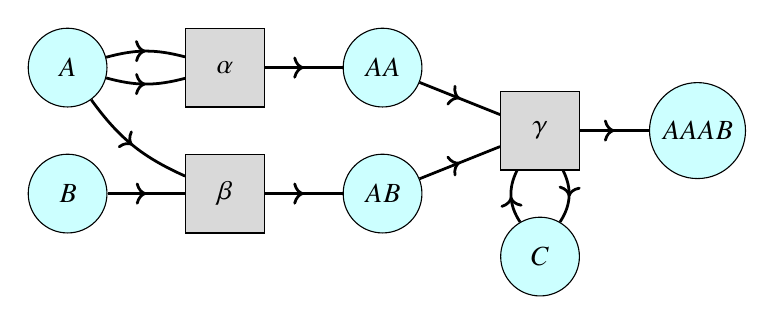
\begin{tikzpicture}
            \begin{pgfonlayer}{nodelayer}
                \node [style=site] (A) at (0, 0.8) {$A$};
                \node [style=site] (B) at (0, -0.8) {$B$};
                \node [style=site] (C) at (6, -1.6) {$C$};
                \node [style=site] (AA) at (4, 0.8) {$AA$};
                \node [style=site] (AB) at (4, -0.8) {$AB$};
                \node [style=site] (AAAB) at (8, 0) {$AAAB$};
                \node [style=transition] (tau1) at (2, 0.8) {$\alpha$};
                \node [style=transition] (tau2) at (2, -0.8) {$\beta$};
                \node [style=transition] (tau3) at (6, 0) {$\gamma$};
            \end{pgfonlayer}
            \begin{pgfonlayer}{edgelayer}
                \draw [style=arrow, bend right=15] (A) to (tau1);
                \draw [style=arrow, bend left=15] (A) to (tau1);
                \draw [style=arrow, bend right=15] (A) to (tau2);
                \draw [style=arrow] (tau1) to (AA);
                \draw [style=arrow] (B) to (tau2);
                \draw [style=arrow] (tau2) to (AB);
                \draw [style=arrow] (AA) to (tau3);
                \draw [style=arrow] (AB) to (tau3);
                \draw [style=arrow, bend left=30] (C) to (tau3);
                \draw [style=arrow] (tau3) to (AAAB);
                \draw [style=arrow, bend left=30] (tau3) to (C);
            \end{pgfonlayer}
        \end{tikzpicture}
    }
\end{center}
then the site $AAAB$ will be terminal and both the initial sites will be $A$, $B$ and $C$.
Sourceless, acyclic Petri nets (nets without loops) will necessarily contain initial sites, and similarly sinkless, acyclic Petri nets will contain terminal sites.

The value of identifying initial sites is that they are necessarily elements of every basis, and if the set of initial sites is a basis in its own right, then it is the only basis.
\begin{lemma}\label{lem:initial-are-basic}
    Let $P$ be a Petri net.
    For any basis $\B$ of $P$, $\Ini{P} \subseteq \B$.
    Furthermore, if $\Ini{P}$ is a basis, then it is a unique basis for $P$.

    \red{I'm not $100\%$ sure of the last point, but I think it's true. We'll find out when we start writing the proof.}

    \green{This is important for internal use. In all of the cases we have dealt with in practice, e.g. molecular assembly as applied, the inital sites form a basis and so there is no ambiguity in the Nat. Comm. paper recently published.}
\end{lemma}
\begin{proof}
    \TODO{Complete}
\end{proof}

Our final concern regaring Petri nets is whether or not bases are are preserved under Petri net morphisms.
To establish that this is the case, we must first show that if two sets of sites are pathway connected, then they will be pathway connected in the image of a Petri net morphism.
\begin{lemma}\label{lem:image-of-pathways}
    Let $f: P \rightarrow Q$ be a Petri net morphism and let $X, Y \subseteq S(P)$ be pathway connected in $P$.
    Then either $f(X)$ and $f(Y)$ are pathway connected in $f(P)$.
\end{lemma}
\begin{proof}
    \TODO{Complete}
\end{proof}

\TODO{Example}

The fact that generating sets are preserved, follows from the preservation of pathways.
\begin{lemma}\label{lem:image-of-generating-sets}
    Let $f: P \rightarrow Q$ be a Petri net morphism and let $X$ be a generating set of $P$.
    Then $f(X)$ is a generating set of $f(P)$.
\end{lemma}
\begin{proof}
    \TODO{Complete}
\end{proof}

\TODO{Example Figure}

This is not to say that the only generating sets in the image of a Petri net will be the image of a generating set.
The codomain of the Petri net morphism may in fact have additional generating sets.

\TODO{Example Figure}

Still, the fact that generating sets are preserved yields nicely our final result: bases are preserved under Petri net morphisms
\begin{corollary}\label{lem:image-basis}
    Let $P$ be a Petri net with basis $\B$ and let $f : A \rightarrow B$ be a Petri net morphism.
    Then $f(\B)$ is a basis for $f(P)$.
\end{corollary}
\begin{proof}
    \TODO{Complete}
\end{proof}
The property that Petri net morphisms preserve bases is fundamentally important for establishing relationships between basis-dependent quantities computed in one Petri net with those in another.

The Petri net formalism, and the extensions presented in this section, can now be leveraged to define the structure of primary interest in this work: assembly spaces.
These spaces can be seen as a subclass of Petri nets which admit specific features useful for describing the fewest number of steps required to construct a given object, the assembly index.
The concepts of subnets and bases will be a key component in the definition of the assembly index, and Petri net morphisms will be indispensible for establishing bounding the value of the assembly index where explict calculation may be infeasible.

\section{Assembly Spaces, Subspaces and Maps}\label{sec:assembly-spaces}

\begin{definition}\label{def:assembly-space}
    An \textbf{assembly space} $(A, \B_A)$ is a sourceless and sinkless Petri net with basis $\B_A$.
    Were possible, we will simply write $A$ to denote an assembly space $(A, \B_A)$.
\end{definition}

\begin{definition}\label{def:assembly-subspace}
    Let $A$ and $A'$ be assembly spaces.
    $A'$ is an \textbf{assembly subspace} of $A$ if $A'$ is a Petri subnet of $A$.
    This relationship is denoted $A' \subseteq A$.
\end{definition}

\begin{definition}\label{def:rooted}
    Let $(A', \B_{A'})$ be an assembly subspace of $(A, \B_A)$.
    We say that $A'$ is rooted in $A$ if $\B_{A'} \subseteq \B_A$.
\end{definition}

\begin{lemma}\label{lem:lower-is-rooted}
    Let $A$ be an assembly space and let $x \in S(A)$.
    Then $\downset{x}$ with basis $\B_A \cap S(\downset{x})$ is a rooted assembly subspace of $A$.
\end{lemma}
\begin{proof}
    \TODO{Complete}
\end{proof}

\begin{definition}\label{def:assembly-map}
    Let $A$ and $B$ be assembly spaces.
    An \textbf{assembly map} is simply a Petri net map $f: A \rightarrow B$ between assembly spaces.
\end{definition}

\begin{theorem}\label{lem:assembly-image-is-subspace}
    If $f : A \rightarrow B$ is an assembly map between assembly spaces $A$ and $B$, then $f(A)$ is an assembly subspace of $B$.
\end{theorem}
\begin{proof}
    \TODO{Complete}
\end{proof}

\begin{theorem}\label{thm:rooted-image}
    Let $A$ be an assembly space, $Z \subseteq A$ a rooted assembly subspace, and $f : A \rightarrow B$ an assembly map.
    Then $(f(Z), S(f)(\B_Z))$ is rooted in $(f(A), S(f)(\B_A)$.
\end{theorem}
\begin{proof}
    \TODO{Complete}
\end{proof}

\section{The Assembly Index}\label{sec:assembly-index}

\begin{definition}\label{def:size}
    Let $A$ be an assembly space.
    The \textbf{size} of $A$ is the cardinality of $T(A)$, denoted $|A|$.
\end{definition}

\begin{definition}\label{def:finiteness}
    Let $A$ be an assembly space and let $x$ be a site in $A$.
    We say that $x$ is \textbf{finite} in $A$ if $\downset{x}$ in $A$ has finite size.
\end{definition}

\begin{definition}\label{def:index}
    Let $A$ be an assembly space and let $x$ be a finite site in $A$.
    The \textbf{assembly index} of $x$ is the minimal size of all rooted assembly subspaces of $A$ containing $x$, and is denoted $c_A(x)$.
    This can be written $c(x)$ when the relevant assembly space is clear from context.
\end{definition}

\subsection{Bounds on the Assembly Index}\label{subsec:assembly-index-bounds}

\begin{theorem}\label{cor:subspace-index-upper-bound}
    Let $(A, \B_A)$ be an assembly space and let $(B, \B_A)$ be a rooted assembly subspace of $A$.
    For every finite $b \in S(B)$, the assembly index of $b$ in $B$ is at least the assembly index of $b$ in $A$.
    That is, $c_B(b) \ge c_A(b)$ for all $b \in S(B)$
\end{theorem}
\begin{proof}
    \TODO{Complete}
    % We need only show that $c_A(b)$ cannot be greater than $c_B(b)$ for any $b \in S(B)$.
    % To see this, let $Z \subseteq B$ be a rooted assembly subspace containing $b$ with $|Z| = c_B(b)$.
    % Then $Z$ is also a rooted assembly subspace of $A$ containing $b$, and so $c_A(b)$ can be at most $|Z|$.
    % That is, $c_A(b) \le |Z| = c_B(b)$.
\end{proof}

\begin{theorem}\label{thm:image-lower-bound}
    If $f: A \rightarrow B$ is an assembly map, then $c_{f(A)}(f(x)) \le c_A(x)$ for all finite $x \in S(A)$.
    Furthermore, if $f$ is an embedding, then $c_{f(A)}(f(x)) = c_A(x)$.
\end{theorem}
\begin{proof}
    \TODO{Complete}
    % Suppose $x \in S(A)$ is finite, and $Z \subseteq A$ is a rooted with $s \in S(Z)$ and $|Z| = c_A(x)$.
    % Restricting $f$ to $Z$ provides an assembly map $f^* : Z \rightarrow B$ such that $f(Z)$ contains $f(x)$, and is rooted in $B$.
    % As such, $c_{f(A)}(f(x))$ can be no larger than $|f(Z)|$, so $c_{f(A)}(f(x)) \le c_A(x)$.
    %
    % Furthermore, suppose that $f$ is an embedding, and consider any $Z' \subseteq f(A)$ rooted and containing $f(x)$.
    % The preimage of $Z'$ under $f$ is then a rooted assembly subspace of $A$ containing $x$, so $c_A(x)$ can be no larger than $|f^{-1}(Z)|$.
    % Together with the previous result, we then have $c_{f(A)}(f(x)) = c_A(x)$.
\end{proof}

\begin{corollary}\label{cor:lowerset-index}
    Let $A$ be an assembly space and $x \in S(A)$ be finite.
    Then $c_A(x) = c_{x\downarrow}(x)$.
\end{corollary}
\begin{proof}
    \TODO{Complete}
    % There is a natural embedding $i : \downset{x} \rightarrow A$, so $c_A(x) = c_{x\downarrow}(x)$ for all finite $x \in S(A)$, as per \cref{thm:image-lower-bound}.
\end{proof}

\subsection{Computability and Algorithms}

\begin{theorem}\label{thm:computable}
    If $A$ is an assembly space and $x \in S(A)$ is finite, then $c(x)$ is computable.
\end{theorem}
\begin{proof}
    \TODO{Complete}
    % Every rooted assembly subspace with minimal size and containing $x$ is a minimal, rooted assembly subspace of $\downset{x}$.
    % Since $x$ is finite, $\downset{x}$ is finite; that is $\downset{x}$ has finitely many transitions.
    % This, together with the fact that $\pi(\sigma(t))$ and $\pi(\tau(t))$ are finite for all $t \in T(A)$, ensures that there areonly finitely many assembly subspaces of $\downset{x}$.
    % As such, the set of all rooted assembly subspaces is computable; simply enumerate them.
    % The size of each subspace is, of course, computable as one need simply count the transitions in the subspace.
    % Finally, finding the minimum value in a finite set of natural numbers is computable.
    % Thus, $c(x)$ is computable.
\end{proof}

\TODO{Typeset split-branch algorithm}

\section{Assembly Examples}

\TODO{Come up with a few fun examples.}

\end{document}
